\documentclass[
  compress
  ,12pt
  %,draft
  %,handout % I don't see how this could ever work for my presentation!
]{beamer}

%%% Unknown packages
%\usepackage{beamerthemesplit}
%\usepackage{times}

% Provides script capital letters for math
\usepackage{mathrsfs}
%\usepackage{verbatim}
\usepackage{subfigure}
\usepackage{amsmath}

\newcommand{\bv}[1]{{\boldsymbol{#1}}}

%%% Fonts. Default font is computer modern
%\usefonttheme{default}
%\usefonttheme{professionalfonts} %allows you to use an external font w/o beamer replacements


%\usefonttheme[onlylarge]{serif}

%%  \usefonttheme[
%%    %onlysmall,
%%    onlylarge
%%    ] {structureitalicserif} %typesets structural text in italics with serifs

%% \usefonttheme[
%%   %onlysmall,
%%   onlylarge
%%   ] {structuresmallcapsserif} %Doesn't look too bad with onlylarge set

 \usefonttheme[
   % stillsansserifmath,
   % stillsansserifsmall,
   % stillsansseriftext,
   onlymath
 ]{serif} %onlymath option doesn't look too bad, eqns are more readable this way.


%%% Font families
%\usepackage{mathptmx} % not avail?
%\usepackage{helvet} % Helvetica is the standard sansserif font if you do not use the serif theme
%\usepackage{avant}   % fat, bubble-like sans serif letters
%\usepackage{chancery} % not available?
%\usepackage{utopia}  % not available?
%\usepackage{charter} % n/a
%\usepackage{times}

% A computer modern font available in T1 encoding.  As far as I
% can tell it doesn't look much different.
%\usepackage{lmodern}
%\usepackage[T1]{fontenc}



%%% Control the position of progress bars, titles, subtitles, etc. 
%\usetheme{default} % No navigation bars!
%\usetheme{boxes} % puts a box a in the head and footline, looks like default unless
                 % you also use \addheadbox and \addfootbox
%\usetheme{Bergen} % huge left-hand column. informal feel
%\usetheme{Boadilla} % shows page count at bottom.  requires institute
%\usetheme{Madrid} % Like Boadilla, but more color contrast
%\usetheme{Pittsburgh} % right-flushed titles, otherwise very sparse
%\usetheme{Rochester}  % Huge title bars dominating the slide. square corners, no drop shadows
%\usetheme{Antibes}     % Large, Tree-based navigation at the top with sharp corners. Not bad
%\usetheme{JuanLesPins}  % Smooth version of Antibes, no lines in nav tree.
%\usetheme{Montpellier}  % To me, it looks like Antibes.  No box backgrounds.
\usetheme{Darmstadt} %fuzzy top title bars, drop shadows, circle bullets,
                     % no side column. The top title is very busy
%\usetheme{Frankfurt}  % fuzzy title bars running across
                      % the top only, circular bullets, drop shadows,
                      % colored blocks with rounded corners, pretty nice
%\usetheme{Warsaw}  % Centrally divided top menu, no progress bullets, top
                   % of the screen is a bit busy but otherwise nice
%\usetheme{Berlin} % Square edges and bullets, no drop shadows, no rounded blocks
%\usetheme{Ilmenau} % Similar to Berlin, mini-nav frame, no drop shadows, rounded corners
%\usetheme{Dresden} % Like Berlin, but no block outlines. minimal context, lots of nav, but not bad
%\usetheme{Darmstadt} % Berlin with no bottom nav and rounded blocks, pretty nice, a bit too much at top though
%\usetheme{Frankfurt} % Very nice! Like Darmstadt but with less nav at the top
%\usetheme{Singapore} % top title bar has a faded appearance, centered title names, minimal bullets.
%\usetheme{Szeged} % Lots of horizontal lines. Pretty nice but too cluttered at the top

% \usetheme{Berkeley} %side-bar menu screws up the spacing of slides somewhat, use with sidebartab
% \usecolortheme{sidebartab} % You really can't have long section names for this one

%\usetheme{Copenhagen} % tabular navigation, flat look (no shadows) too much top clutter
%\usetheme{Malmoe} % top cluttered
%\usetheme{Luebeck} % top cluttered
%\usetheme{Warsaw} % top is cluttered and even has a drop shadow


% \usetheme{Goettingen} % Looks like Berkely, but less obtrusive nav bar is on the right
% \usecolortheme{sidebartab} % Used with sidebartab, it's really not bad

%\usetheme{Marburg} % A more dominant Goettingen, harder to read sidebar

%\usetheme{Hannover} % right flush titles, left-side nav, top looks a little empty

% This color theme works with all themes that show a table of contents in the sidebar.
\usecolortheme{sidebartab} 

%%% Color Themes: Make your colors bolder or more muted
%\usecolortheme{seahorse} % outer color theme, muted grey, a really nice one!, use with rose
                          % or lilly inner color themes
%\usecolortheme{rose}      % dark blue with relatively stark constrast levels
%\usecolortheme{lily}       % as above, but blocks do not have backround color
\usepackage{times}
\usepackage{units}

\setbeamercovered{invisible}
%\logo{\includegraphics[width=.5in]{figures/word3}}
%\setbeamercolor{title}{fg=red!80!black,bg=red!20!white}

\title{Adaptive FEM for Applications}
\author{John W.\ Peterson \\ \texttt{\tiny peterson@cfdlab.ae.utexas.edu}}
\institute[UT-Austin]{Univ.\ of Texas at Austin}
\date{January 12, 2007}

% Re-show the TOC at the beginning of each section
\AtBeginSection[]{\frame{\tableofcontents[current]}}

\setbeamercovered{transparent}


\newcommand{\R}{\mathscr{R}}

\begin{document}


  
\begin{frame}
  \titlepage
\end{frame}

% An Outline Slide
%\section[Outline]{}
%\frame{\tableofcontents[pausesections]}

\section{Linearized Shallow Water Equations}
\begin{frame}[t]
  \frametitle{Physical Setup}
  \begin{center}
  \includegraphics[width=.4\textwidth,angle=-90]{figures/sw_define}
  \end{center}
      \begin{itemize}
      \item
	{
	 Total Elevation $h=H+\eta$ 
	}
      \item
	{
	  $\eta \ll H$
	}
      \end{itemize}
\end{frame}

\begin{frame}
  \frametitle{Governing Equations}
  \begin{eqnarray}
    %\label{eqn:nlmomentum}
    \nonumber
    \frac{\partial \bv{u}}{\partial t}
    \only<1-2>
    {
      + \alert<2>{(\bv{u} \cdot \nabla) \bv{u}}
    }
    + f \bv{k}\times \bv{u} + g \nabla \eta &=& 0 \\
    %\label{eqn:nlelevation}
    \nonumber
    \frac{\partial \eta}{\partial t} +
    \nabla \cdot \left[
      \only<1-4>
      {
	(\alert<4>{H + \eta}) \bv{u}
      }
      \only<5-6>
      {
	\alert<5>{H} \bv{u}
      }
      \right]  &=& 0
  \end{eqnarray}
  \begin{itemize}
    \item {$f=2\varOmega\sin\varPhi$ is the Coriolis parameter}
    \item {$g$ is gravity}
  \end{itemize}
\end{frame}


\begin{frame}%[t]
  \frametitle{Relation to 2nd-order Wave Equation}
  \begin{itemize}
    \item{Let $f=0$ and assume 1D flow, $H=H(x)$}
    \item{
      Letting $w := Hu$, we obtain
      \begin{equation}
	\nonumber
	w_{tt} - gH w_{xx} = 0
      \end{equation}
    }
    \item{So $gH$ is like a (spatially-varying) wave speed}
  \end{itemize}
\end{frame}


\begin{frame}%[t]
  \frametitle{Variational Statement}
  \begin{itemize}
    \item{Find $\{\bv{u}, \eta\}$ such that}
  \end{itemize}
  \begin{eqnarray}
    \nonumber
    %\label{eqn:momentum_weak}
    \int_{\Omega}
    \left(
    \frac{\partial \bv{u}}{\partial t} + f \bv{k}\times \bv{u} + g \nabla \eta
    \right) \cdot \bv{\phi} \;dx &=& 0 \\
    \nonumber
    %\label{eqn:elevation_weak}
    \int_{\Omega}
    \frac{\partial \eta}{\partial t}\psi - H \left( \bv{u} \cdot \nabla \psi \right)\;dx
    + \int_{\partial \Omega} H \left( \bv{u} \cdot \bv{n} \right) \psi \;ds &=& 0
  \end{eqnarray}
  holds for every admissible $\{\bv{\phi}, \psi\}$
\end{frame}

\begin{frame}%[t]
  \frametitle{Finite Element Approximations}
  \begin{itemize}
    \item{Many different finite element pairs have been tried \ldots}
    \item{
  \only<1>
      {
	$P_1^{NC}-P_1$
	\begin{center}
	  \includegraphics[width=.4\textwidth,angle=-90]{figures/P1NCP1}
	\end{center}
      }
      %
%%   \only<2>
%%       {
%% 	$P_2-P_1$
%% 	\begin{center}
%% 	  \includegraphics[width=.4\textwidth,angle=-90]{figures/P2P1}
%% 	\end{center}
%%       }
      %
  \only<2>
      {
	$P_1-P_1$
	\begin{center}
	  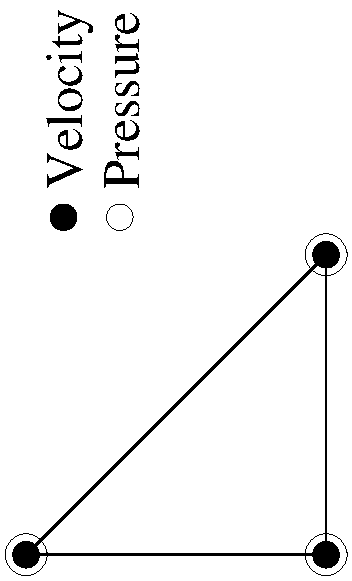
\includegraphics[width=.4\textwidth,angle=-90]{figures/P1P1}
	\end{center}
      }
      %
  \only<3>
      {
	$P_0-P_1$
	\begin{center}
	  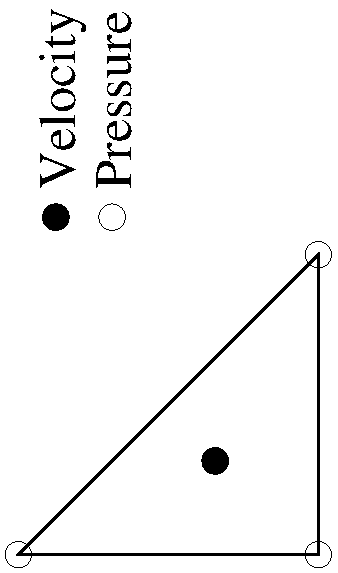
\includegraphics[width=.4\textwidth,angle=-90]{figures/P0P1}
	\end{center}
      }
%%   \only<5>
%%       {
%% 	$RT0$
%% 	\begin{center}
%% 	  \includegraphics[width=.4\textwidth,angle=-90]{figures/RT0}
%% 	\end{center}
%%       }
    }
  \end{itemize}
\end{frame}


\begin{frame}%[t]
  \frametitle{FE-pair advantages/disadvantages}
  \begin{itemize}%[<+->]
%  \item{Each FE-pair has various advantages/disadvantages, for example}
    \only<1>
    {
    \item{
      $P_1^{NC}-P_1$
      \begin{itemize}
	\item {$+$ ``A promising choice for the discretization of a variety
	  of coastal and environmental problems'' (Le~Roux, 2005)}
	\item {$-$ Difficult to use in $h$-adaptive codes with hanging nodes and
	  nested spaces}
      \end{itemize}
      }
      }
    \only<2>
    {
    \item{
      $P_1-P_1$
      \begin{itemize}
	\item {$+$ Simple implementation, elements work fine in $h$-adaptive codes}
	\item {$-$ ``Spurious modes of wavelength $3h$ are present'' for gravity
	  wave propagation problems with non-constant bathymetry (Le~Roux, 2007)}
	\item{$-$ ``the $P_1-P_1$ pair is usually not used to solve the SW system, unless
	  \ldots a stabilization procedure is employed'' (\emph{ibid})}
      \end{itemize}
      }
      }
    \only<3>
    {
    \item{
      $P_0-P_1$
      \begin{itemize}
	\item {$+$ No spurious elevation modes as for $P_1-P_1$}
	\item {$-$ Actually \emph{more} expensive than $P_1-P_1$ on an equivalent mesh}
	\item {$-$ Only weak enforcement of velocity BCs is possible since there are no
	  velocity dofs on the element edges}
      \end{itemize}
      }
      }
  \end{itemize}
\end{frame}

\begin{frame}%[t]
  \frametitle{Rossby Wave Propagation}
  \begin{itemize}[<+->]
  \item{Rossby waves are large-scale motions in the ocean or atmosphere}
  \item{Caused by e.g.\ meanders of the jet (or gulf) stream}
  \item{Cold fronts}
  \item{In the ocean, waves can take months or years to cross the Pacific ocean}
  \item{Long-time simulations must avoid adding too much artificial dissipation}
  \end{itemize}
\end{frame}


\begin{frame}%[t]
  \frametitle{Rossby Wave Propagation}
  \begin{itemize}%[<+->]
  \item{We can model Rossby waves with the linearized SW equations.}
  \item{The Coriolis term is linearized around a particular latitude value as
  \begin{equation}
    \nonumber
    f = f_0 + \beta y
  \end{equation}
  }
  \item{$f_0=6.16 \times 10^{-5}$ 1/s}
  \item{$\beta = 2.07 \times 10^{-11}$ m/s}
  \end{itemize}
\end{frame}

\begin{frame}%[t]
  \frametitle{Rossby Wave Propagation}
  \begin{itemize}%[<+->]
  \item{The initial condition is a Gaussian that satisfies the linear
    SW equations with $\beta=0$.
    }
  \end{itemize}
  \begin{eqnarray}
    \nonumber
    \bv{u}_0 &=&  2 \frac{g}{f_0} a b  e^{-b \left(x^2+y^2\right)}\left(y,-x\right) \\
    \nonumber
    \eta_0   &=&  a e^{-b \left(x^2+y^2\right)}
  \end{eqnarray}
  \begin{itemize}
    \item{Problem is posed in a rectangular domain of physical
      size 2000 km $\times$ 1200 km.
%%       domain size:
%%       \begin{equation}
%% 	\nonumber
%% 	(x,y) \in [-1000,1000]\times[-600,600] \text{ km}
%%       \end{equation}
    }
  \end{itemize}
\end{frame}

\begin{frame}[t]
  \frametitle{Initial Condition, $|\bv{u}_0|$}
\vspace{-0.2in}
  \begin{center}
    \includegraphics[width=.9\textwidth]{figures/P0P1_velocity_0000}
  \end{center}
\end{frame}

\begin{frame}[t]
  \frametitle{Initial Condition, $\eta_0$}
\vspace{-0.2in}
  \begin{center}
    \includegraphics[width=.9\textwidth]{figures/P0P1_elevation_0000}
  \end{center}
\end{frame}

\include{P0P1_results}


\begin{frame}[t]
  \frametitle{$P_1-P_1$ elements, $|\bv{u}|$ at $t\approx 5.55$hr}
\vspace{-0.2in}
  \begin{center}
    \includegraphics[width=.9\textwidth]{figures/P1P1_velocity_0020}
  \end{center}
\end{frame}

\begin{frame}[t]
  \frametitle{$P_1-P_1$ elements, $\eta$ at $t\approx 5.55$hr}
\vspace{-0.2in}
  \begin{center}
    \includegraphics[width=.9\textwidth]{figures/P1P1_elevation_0020}
  \end{center}
\end{frame}


\begin{frame}[t]
  \frametitle{Stabilized Formulation}
  \begin{itemize}[<+->]
  \item{We can write the linearized SW equations in the standard notation
    for systems
    \begin{equation}
  \nonumber
  \frac{\partial \bv{U}}{\partial t}
  + \bv{A}_i\frac{\partial \bv{U}}{\partial x_i}
  + \bv{C} \bv{U}
  = 0
  \end{equation}
  }

    \item{Where
\begin{equation}
  \nonumber
  \hspace{-.5in}
  \bv{A}_1 = \begin{bmatrix}
    \begin{array}{ccc}
      \alert<3>{0} & 0 & g  \\
      0 & \alert<3>{0} & 0  \\
      H & 0 & \alert<3>{0} 
    \end{array}
  \end{bmatrix}
  \hspace{.1in}
  \bv{A}_2 = \begin{bmatrix}
    \begin{array}{ccc}
      \alert<3>{0} & 0 & 0  \\
      0 & \alert<3>{0} & g  \\
      0 & H & \alert<3>{0} 
    \end{array}
  \end{bmatrix}
  \hspace{.1in}
  \bv{C} = \begin{bmatrix}
    \begin{array}{ccc}
      0 & -f & 0  \\
      f & 0 & 0  \\
      \partial_x H & \partial_y H & 0 
    \end{array}
  \end{bmatrix}
\end{equation}
      }
  \end{itemize}
\end{frame}


\begin{frame}[t]
  \frametitle{Stabilized Formulation -- Var.\ Stmt.}
  \begin{itemize}
    \item{Using system notation, the variational statement is:
      Find $\bv{U}\only<2>{\alert{^h}}$ s.t.
      \begin{equation}
	\nonumber
	\int_{\Omega} \left( \frac{\partial \bv{U}\only<2>{\alert{^h}}}{\partial t}
	+ \bv{A}_i\frac{\partial \bv{U}\only<2>{\alert{^h}}}{\partial x_i}
	+ \bv{C} \bv{U}\only<2>{\alert{^h}} \right) \cdot \bv{W}\only<2>{\alert{^h}} \;dx
	= 0
      \end{equation}
      holds for every admissible $\bv{W}\only<2>{\alert{^h}}$.
    }
      \only<2>
	  {
	    \item{
	    The approximate problem is obtained by replacing the continuous
	    variables with their FE approximations,
	    $\bv{U}^{\alert{h}}$ and $\bv{W}^{\alert{h}}$.}
	  }
  \end{itemize}
\end{frame}

\begin{frame}[t]
  \frametitle{Stabilized Formulation -- Var.\ Stmt.}
  \begin{itemize}[<+->]
    \item{The stabilized FE formulation then becomes:
      Find $\bv{U}^h$ s.t.
      \begin{eqnarray}
  \nonumber
  \int_{\Omega} \left( \frac{\partial \bv{U}^h}{\partial t}
  + \bv{A}_i\frac{\partial \bv{U}^h}{\partial x_i}
  + \bv{C} \bv{U}^h \right) \cdot \bv{W}^h \;dx &+&
  \\
  \nonumber
  \int_{\Omega'} \bv{A}_i\frac{\partial \bv{W}^h}{\partial x_i}
  \cdot \bv{\tau} \left( \frac{\partial \bv{U}^h}{\partial t}
  + \bv{A}_i\frac{\partial \bv{U}^h}{\partial x_i}
  + \bv{C} \bv{U}^h \right)dx 
  &=& 0
\end{eqnarray}
      holds for every admissible $\bv{W}^h$.
    }
    \item{This is a standard SUPG-type stabilization scheme}
    \item{$\bv{\tau}$ is a matrix of stabilization parameters}
  \end{itemize}
\end{frame}

\begin{frame}[t]
  \frametitle{SUPG Operator}
  \begin{itemize}%[<+->]
    \item{The SUPG operator is: 
      \begin{equation}
	\nonumber
   \bv{A}_i\frac{\partial \bv{W}^h}{\partial x_i} =
   \begin{bmatrix}
     \renewcommand{\arraystretch}{1.3}
     \begin{array}{c}
       g \frac{\partial \psi^h}{\partial x} \\
       g \frac{\partial \psi^h}{\partial y} \\
       H \left( \nabla \cdot \bv{\phi}^h \right) \\
     \end{array}
   \end{bmatrix}
\end{equation}
      }

    \item{
      We employ a particularly simple form of $\bv{\tau}$:
\begin{equation}
  \nonumber
\bv{\tau} = diag(\tau_{11}, \tau_{22}, \tau_{33})
\end{equation}
    }
  \end{itemize}
\end{frame}


\begin{frame}[t]
  \frametitle{Stabilization Parameters}
  \begin{itemize}%[<+->]
    \item{The stabilization parameters are chosen based on
      the work of Shakib et al.
      \begin{equation}
	\nonumber
  \bv{\tau} = \left(
  \frac{\partial \xi_i}{\partial x_j}
  \frac{\partial \xi_i}{\partial x_k}
  \bv{A}_j\bv{A}_k 
\right)^{-1/2}
      \end{equation}
      }
      \item{Where
	\begin{equation}
	  \nonumber
	  \frac{\partial \xi_i}{\partial x_j} \propto \frac{1}{h}
	\end{equation}
	is the $(i,j)^{th}$ entry of the element
Jacobian matrix.}
  \end{itemize}
\end{frame}

\begin{frame}[t]
  \frametitle{Stabilized Equations}
  \begin{itemize}%[<+->]
  \item{The stabilized momentum equations are then:
    \begin{eqnarray}
      \nonumber
      \int_{\Omega}
      \left(
      \frac{\partial \bv{u}^h}{\partial t} + f \bv{k}\times \bv{u}^h + g \nabla \eta^h
      \right) \cdot \bv{\phi}^h \;dx
      &+& \\
      \nonumber
      \int_{\Omega'}
      \alert<2>{\tau_{33}
	}
      \alert<3>{
      H \left(\nabla \cdot \bv{\phi}^h\right)
      }
      \left( \alert<4>{
	\frac{\partial \eta^h}{\partial t} +
	\nabla \cdot (H \bv{u}^h)
	}
      \right) \;dx
      &=& 0 
  \end{eqnarray}
    }
    
    \only<2>
    {
      \item{Stabilization parameter}
    }
    \only<3>
    {
      \item{SUPG operator}
    }

    \only<4>
    {
      \item{Elevation equation ``residual''}
    }
  \end{itemize}
\end{frame}


\begin{frame}[t]
  \frametitle{Stabilized Equations}
  \begin{itemize}%[<+->]
  \item{While the stabilized elevation equation is:
    \begin{eqnarray}
    \nonumber
    \int_{\Omega}
    \frac{\partial \eta^h}{\partial t}\psi^h -
    H \left( \bv{u}^h \cdot \nabla \psi^h \right)\;dx
    + \int_{\partial \Omega} H \left( \bv{u}^h \cdot \bv{n} \right) \psi^h \;ds &+& \\
    \nonumber
    \int_{\Omega'} \alert<3>{g}
    \left[\alert<2>{\tau_{11}}
      \alert<3>{\frac{\partial \psi^h}{\partial x}},
      \alert<2>{\tau_{22}}
      \alert<3>{\frac{\partial \psi^h}{\partial y}}
      \right]^t \cdot 
    \left(
      \alert<4>{\frac{\partial \bv{u}^h}{\partial t} +
      f \bv{k}\times \bv{u}^h + g \nabla \eta^h
      }
    \right)
    \;dx &=& 0
  \end{eqnarray}
    }
    
    \only<2>
    {
      \item{Stabilization parameters}
    }
    \only<3>
    {
      \item{SUPG operator}
    }

    \only<4>
    {
      \item{Momentum equation ``residual''}
    }
  \end{itemize}
\end{frame}


\begin{frame}[t]
  \frametitle{$P_1-P_1$ stab, $|\bv{u}|$ at $t\approx 5.55$hr}
\vspace{-0.2in}
  \begin{center}
    \includegraphics[width=.9\textwidth]{figures/P1P1_full_supg_velocity_0020}
  \end{center}
\end{frame}

\begin{frame}[t]
  \frametitle{$P_1-P_1$ stab, $\eta$ at $t\approx 5.55$hr}
\vspace{-0.2in}
  \begin{center}
    \includegraphics[width=.9\textwidth]{figures/P1P1_full_supg_elevation_0020}
  \end{center}
\end{frame}

\begin{frame}[t]
  \frametitle{Full SUPG results}
  \begin{itemize}
    \item{Initial results are stable, but much too diffusive}
    \item{Peak $|\bv{u}|$ is roughly 40\% of the $P_0-P_1$ result}
  \end{itemize}
  \vspace{-.2in}
  \begin{center}
%%   \includegraphics[width=.45\textwidth]{figures/P0P1_velocity_0020}
%%   \includegraphics[width=.45\textwidth]{figures/P1P1_full_supg_velocity_0020}
    \includegraphics[width=.8\textwidth]{figures/P0P1_P1P1_cutlines}
  \end{center}
\end{frame}

\begin{frame}[t]
  \frametitle{``Half-SUPG'' Method}
  \begin{itemize}[<+->]
    \item{
      One successful attempt to reduce the amount of artifical diffusion
      present was to set $\tau_{11}=\tau_{22}=0$
    }
    \item{This means only the momentum equations are stabilized, the
      elevation equation is solved using standard Galerkin}
    \item{The results appear to be better, but they are still preliminary
      (we cannot explain why yet)}
    \item{Similar to the so-called GLS scheme sometimes employed to
      allow equal-order approximation spaces for the Stokes equations}
  \end{itemize}
\end{frame}


\begin{frame}[t]
  \frametitle{Half-SUPG results}
%%   \begin{itemize}
%%     \item{Initial results are stable, but much too diffusive}
%%     \item{Peak $|\bv{u}|$ is roughly 40\% of the $P_0-P_1$ result}
%%   \end{itemize}
%%   \vspace{-.2in}
  \begin{center}
    \includegraphics[width=.8\textwidth]{figures/P0P1_P1P1_half_cutlines}
  \end{center}
\end{frame}

\begin{frame}[t]
  \frametitle{Adaptive Half-SUPG results}
%%   \begin{itemize}
%%     \item{Initial results are stable, but much too diffusive}
%%     \item{Peak $|\bv{u}|$ is roughly 40\% of the $P_0-P_1$ result}
%%   \end{itemize}
%%   \vspace{-.2in}
  \begin{itemize}
    \item{The method also appears promising with AMR}
  \end{itemize}
  \vspace{-.2in}
  \begin{center}
    \includegraphics[width=.8\textwidth]{figures/P0P1_P1P1_half_AMR_cutlines}
  \end{center}
\end{frame}

\begin{frame}[t]
  \frametitle{Adaptive Half-SUPG results}
\vspace{-0.2in}
  \begin{center}
    \only<1>
    {
      \includegraphics[width=.9\textwidth]{figures/P1P1_tau11_tau22_zero_adaptive_velocity_0020}
    }
    \only<2>
    {
      \includegraphics[width=.9\textwidth]{figures/P1P1_tau11_tau22_zero_adaptive_elevation_0020}
    }
    \only<3>
    {
      \includegraphics[width=.9\textwidth]{figures/P1P1_tau11_tau22_zero_adaptive_mesh_0020}
    }
  \end{center}
\end{frame}


\begin{frame}[t]
  \frametitle{\ldots And Higher-Order $\left(P_2-P_2\right)$ Elements}
\vspace{-0.2in}
  \begin{center}
    \only<1>
    {
      \includegraphics[width=.9\textwidth]{figures/P2P2_tau11_tau22_zero_adaptive_velocity_0020}
    }
    \only<2>
    {
      \includegraphics[width=.9\textwidth]{figures/P2P2_tau11_tau22_zero_adaptive_elevation_0020}
    }
    \only<3>
    {
      \includegraphics[width=.9\textwidth]{figures/P2P2_tau11_tau22_zero_adaptive_mesh_0020}
    }
  \end{center}
\end{frame}



\begin{frame}[t]
  \frametitle{Computational Expense}
  \begin{center}
    \renewcommand{\arraystretch}{1.2}
    \begin{tabular}{|c|r|r|r|} \hline
                     &  N.~nodes & N.~cells &  N.~DOFs \\ \hline
    Uniform  $P_0-P_1$  &  9,386    & 18,450   &  46,286  \\ \hline
    Uniform  $P_1-P_1$  &  9,386    & 18,450   &  28,158  \\ \hline
    Adaptive $P_1-P_1$  &  17,151   & 29,946   &  51,453  \\ \hline
    Adaptive $P_2-P_2$  &  18,453   & 8,878    &  55,359 \\ \hline
  \end{tabular}
  \end{center}
  \begin{itemize}
    \item{Comparison of problem size at a representative timestep}
    \item{AMR is also more expensive because you have to compute error indicators, etc.}
  \end{itemize}
\end{frame}

\begin{frame}
  \frametitle{Future Work}
  \begin{itemize}
  \item{Analytical dispersion analysis of the proposed ``half''-SUPG scheme}
  \item{Additional simulations of non-constant bathymetry problems}
  \item{Tweaked selection of stabilization parameters}
  \end{itemize}
\end{frame}



\section{Double-Diffusive Convection in Porous Media} 
\include{dd_intro}
\begin{frame}
      \begin{itemize}
      \item{
	The problem of determining the Sherwood number can be thought of generically.}

      \item{
	We consider the integrated flux $I$ of some variable $u$ through
	a boundary $\Gamma \subseteq \partial \Omega$

	\begin{equation}
	  \nonumber
	  I := \int_{\Gamma} k \nabla u \cdot n \;ds = -\int_{\Gamma} \sigma \cdot n \;ds 
	\end{equation}
      }
        
      \item{For example, $I$ could be total mass/thermal flux, Lift, Drag, etc.}

      \item{Differentiating the FE solution
	%to obtain $\sigma\cdot n$ is only
	%$\mathcal{O}(h^p)$ accurate.
	generally yields 
	\begin{equation}
	  \nonumber
	  \| \sigma - \sigma_h \|_{L_2(\Gamma)} \approx \mathcal{O}(h^p)
	\end{equation}
      } 
	
      \end{itemize}
\end{frame}


\begin{frame}
  \frametitle{S.~C.~Boundary Flux Literature}
      \begin{itemize}
      \item
	{
          Many schemes for computing superconvergent boundary fluxes have been investigated:

	  \begin{itemize}
	  \item{J.~Douglas, T.~Dupont, and M.~Wheeler (1974)}
	  \item{M.~Wheeler (1979)}
	  \item{Carey et al. (1982, 2002)}
	  \item{Hughes, Larson, Cochburn, Wahlbin, Babu{\v{s}}ka, \ldots}
	  \end{itemize}
	}
	
      \item{Under some restrictions
	\begin{equation}
	  \nonumber
	  \| \sigma - \sigma_h \|_{L_2(\Gamma)} \approx \mathcal{O}(h^{p+1})
	\end{equation}

	is generally possible, see e.g.\ Douglas.}
	
      \end{itemize}
\end{frame}


\begin{frame}
  \frametitle{Model Problem: Poisson}
	\begin{equation}
	  \nonumber
	  -\nabla \cdot \left( k \nabla u \right)=f
	\end{equation}
      \begin{itemize}
      \item<1->{For all $\phi_i \neq 0$ on $\partial \Omega$
      \begin{equation}
	\nonumber
	-\int_{\partial \Omega} \left( \sigma\only<2->{\alert<2>{_h}} \cdot n\right)\phi_i \;ds =
	\int_{\Omega} k\nabla u\only<2->{\alert<2>{_h}} \cdot \nabla \phi_i - f\phi_i \;dx 
	\end{equation}

      }
	
      \item<3->{Can use this relation to solve for improved flux approximation.}

      \item<4->{Difficulties \ldots
	\begin{itemize}
	  \item {$\sigma \cdot n$ discontinuous at a node}
	  \item {$n$ not well-defined at nodes}
	  \item {3D extension}
	\end{itemize}
      }
      \end{itemize}
\end{frame}




\begin{frame}
      \begin{itemize}
      \item{
        It's simpler if we don't care about pointwise values of $\sigma \cdot n$,
	i.e.\ only the integrated flux is
	important.}

      \item{Carey (2002) uses partition of unity method: on $\partial \Omega$,
	\begin{equation}
	  \nonumber
	  \sum_{i=1}^N \phi_i = 1
	\end{equation}
	where $N$ is the number of nodes on $\partial \Omega$, to show that
	\begin{eqnarray}
	  \nonumber
	  -\int_{\partial \Omega} \left(\sigma_h \cdot n\right)
	   \underbrace{\left(\sum_{i=1}^N \phi_i \right)}_{=1} ds &=&
	\sum_{i=1}^N \int_{\Omega} k\nabla u_h \cdot \nabla \phi_i - f\phi_i \;dx
	%\\
	%I &=& \sum_{i=1}^N \int_{\Omega} k\nabla u_h \cdot \nabla \phi_i - f\phi_i \;dx 
	\end{eqnarray}
      }
      \end{itemize}
\end{frame}




\begin{frame}
      \begin{itemize}
      \item{
        We can do something similar on $\Gamma \subset \partial \Omega$: let $S$ be the set of elements
	which have a node on $\Gamma$, and let
	\begin{equation}
	  \nonumber
	  \sum_{i=1}^M \phi_i = 1 
	\end{equation}
	on $\Gamma$ where $M$ is the number of nodes on $\Gamma$.
	%, and $\Gamma_{+}$ is a slightly
	%larger domain.
      }
	
      \item{
	Then we have
	\begin{eqnarray}
	  \nonumber
	  \sum_{i=1}^M \int_{\Gamma_{+}}-\left(\sigma_h\cdot n\right)  \phi_i \;ds =
	  \sum_{i=1}^M \int_{S} k\nabla u_h \cdot \nabla \phi_i - f\phi_i \;dx 
	\end{eqnarray}
      }
      \end{itemize}
\end{frame}


\begin{frame}
  \begin{center}
    \includegraphics[width=.4\textwidth,angle=-90]{figures/square}    
  \end{center}

      \begin{itemize}
      \item{
        Example: $\Gamma$ is the bottom side, $\Gamma_{+}$ extends into the first element
	of the two adjacent sides.
	}
      \end{itemize}
\end{frame}





\begin{frame}
      \begin{itemize}
      \item{We can rewrite this as, let $ q_h  := -\left(\sigma_h \cdot n\right)$
	\begin{eqnarray}
	  \nonumber
	  \sum_{i=1}^M \int_{\Gamma} q_h \phi_i ds +
	  \int_{\Gamma_{+} \setminus \Gamma} \!\!\!\!\!\!\! q_h \phi_1 ds +
	  \int_{\Gamma_{+} \setminus \Gamma} \!\!\!\!\!\!\! q_h \phi_M ds 
	  &=&\\
	  \nonumber
	  \sum_{i=1}^M \int_{S} k\nabla u_h \cdot \nabla \phi_i - f\phi_i \;dx 
	\end{eqnarray}
	or,
	\begin{eqnarray}
	  \nonumber
	  I_h  &=&
	  \sum_{i=1}^M \int_{S} k\nabla u_h \cdot \nabla \phi_i - f\phi_i \;dx -
	  \int_{\Gamma_{+} \setminus \Gamma} \!\!\!\!\!\!\! q_h \phi_1 ds -
	  \int_{\Gamma_{+} \setminus \Gamma} \!\!\!\!\!\!\! q_h \phi_M ds 
	\end{eqnarray}
	}

      \item{If $\Gamma_{+} \setminus \Gamma$ is a Neumann boundary, the extra terms on the r.h.s.\
	are known.  In general the extra terms aren't known.}
      \end{itemize}
\end{frame}

\begin{frame}
  \frametitle{Application to D.~D.\ Convection}
  \begin{itemize}
    \item{ We now proceed to use the flux formula to
      compute Sherwood numbers for the double-diffusion problem
      \vspace{-.2in}
      \begin{center}
	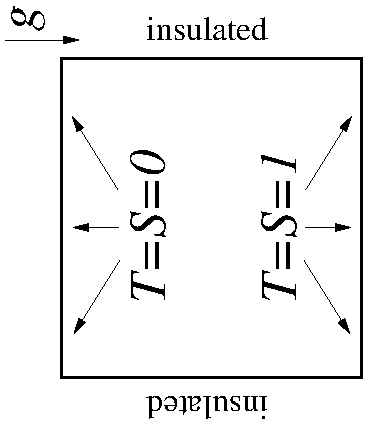
\includegraphics[width=.3\textwidth,angle=-90]{figures/setup}
      \end{center}
    }
    \item{The goal is to compute the steady state value of 
      $I := -\int\nabla S \cdot n \;dx$ or $-\int\nabla T \cdot n \;dx$
      at the bottom (or top) of the enclosure.}
  \end{itemize}
\end{frame}



\begin{frame}
  \frametitle{Application to D.~D.\ Convection}
  \begin{itemize}
    \item{As a simple test problem, we consider the case $\kappa=1$.}
    \item{In this case, $T=S$ at steady state so it suffices to consider
      the flux of only a single variable. }
  \end{itemize}
\end{frame}

\begin{frame}
  \frametitle{Application to D.~D.\ Convection}
    \vspace{-.25in}
    \begin{center}
	\includegraphics[width=.8\textwidth]{figures/kappa1_solute_error_bilinears.pdf}    
  \end{center}
    \vspace{-.2in}
    \begin{itemize}
      \item{Surprisingly, the classical method is actually \emph{better} here.}
    \end{itemize}
\end{frame}

\begin{frame}
  \frametitle{Application to D.~D.\ Convection}\vspace{-.25in}
    \begin{center}
	\includegraphics[width=.8\textwidth]{figures/kappa1_solute_error_biquadratics.pdf}    
  \end{center}
\vspace{-.2in}
    \begin{itemize}
      \item{For biquadratics, the boundary flux formula recovers the $p+1$ rate.}
    \end{itemize}
\end{frame}

\begin{frame}
  \frametitle{$h$-Adaptivity (small $\kappa$ case)}
  \begin{itemize}
    \item{We now employ an extremely simple flux jump error estimator to drive adaptivity
  \begin{equation}
    \nonumber
    \eta^{\text{FLUX}}_K := \left( {h_K} \int_{\partial K} |R_K|^2 ds \right)^{1/2}
    \label{eqn:flux_indicator}
  \end{equation}
  }

    \item{
where $R_K$ is the local residual defined by
\begin{equation}
  \nonumber
  R_K := \left\{
    \begin{array}{cl}
      0, & s \in \partial K \cap \Gamma_D \\
      g_N - \nabla u_h \cdot n_K, & s \in \partial K \cap \Gamma_N \\
      \frac{1}{2}(\nabla u_h|_L - \nabla u_h|_K) \cdot n_K, & s \in \partial K \cap \partial L \neq \emptyset
    \end{array}
    \right.
  \label{eqn:residual}
\end{equation}
%% where $g_N$ is given Neumann boundary data, $n_K$ is the outward unit
%% normal for cell $K$, and cell $L$ shares an edge (face) with cell $K$
%% in the finite element mesh.
}
  \end{itemize}
\end{frame}


\begin{frame}
  \frametitle{Biquadratic Adaptivity}
  \begin{center}
	\includegraphics[width=.8\textwidth]{figures/biquad_amr_0000}    
  \end{center}
\end{frame}
  
\begin{frame}
  \frametitle{Biquadratic Adaptivity}
  \begin{center}
	\includegraphics[width=.8\textwidth]{figures/biquad_amr_0001}    
  \end{center}
\end{frame}

  \begin{frame}
  \frametitle{Biquadratic Adaptivity}
  \begin{center}
	\includegraphics[width=.8\textwidth]{figures/biquad_amr_0002}    
  \end{center}
\end{frame}
\begin{frame}
  \frametitle{Biquadratic Adaptivity}
  \begin{center}
	\includegraphics[width=.8\textwidth]{figures/biquad_amr_0003}    
  \end{center}
\end{frame}
\begin{frame}
  \frametitle{Biquadratic Adaptivity}
  \begin{center}
	\includegraphics[width=.8\textwidth]{figures/biquad_amr_0004}    
  \end{center}
\end{frame}
\begin{frame}
  \frametitle{Biquadratic Adaptivity}
  \begin{center}
	\includegraphics[width=.8\textwidth]{figures/biquad_amr_0005}    
  \end{center}
\end{frame}
\begin{frame}
  \frametitle{Biquadratic Adaptivity}
  \begin{center}
	\includegraphics[width=.9\textwidth]{figures/biquad_adapt_vs_unif_thermal}    
  \end{center}
\end{frame}
\begin{frame}
  \frametitle{Biquadratic Adaptivity}
  \begin{center}
	\includegraphics[width=.9\textwidth]{figures/biquad_adapt_vs_unif_solute}    
  \end{center}
\end{frame}






\begin{frame}
  \frametitle{Future Work}
  \begin{itemize}
    \item{Improved (practical) error indicators}
    \item{Explain higher-than-expected accuracy of classical
      flux calculation for bilinear elements} 
  \end{itemize}
\end{frame}


\end{document}

% LocalWords:  rcl fv Nonlinearity pausesections nd Hu tt gH bathymetry BCs
% LocalWords:  Rossby
